\documentclass{beamer}
\setbeamertemplate{itemize items}[ball]

\usepackage{listings}
\usepackage{xcolor}
\usepackage{multicol}
\usepackage{amsmath}
\usepackage{subcaption}

\definecolor{codegreen}{rgb}{0,0.6,0}
\definecolor{codegray}{rgb}{0.5,0.5,0.5}
\definecolor{codepurple}{rgb}{0.58,0,0.82}
\definecolor{backcolour}{rgb}{0.95,0.95,0.92}

\lstdefinestyle{mystyle}{
    %backgroundcolor=\color{backcolour}, 
    commentstyle=\color{codegreen},
    keywordstyle=\color{magenta},
    numberstyle=\tiny\color{codegray},
    stringstyle=\color{codepurple},
    basicstyle=\ttfamily\footnotesize,
    breakatwhitespace=false,         
    breaklines=true,                 
    captionpos=b,                    
    keepspaces=true,                 
    numbers=left,                    
    numbersep=5pt,               
    showspaces=false,
    showstringspaces=false,
    showtabs=false,                  
    tabsize=2
}

\lstset{style=mystyle}

\usepackage{hyperref}
\hypersetup{
    colorlinks=true,
    linkcolor=blue,
    filecolor=magenta,      
    urlcolor=cyan
}

\urlstyle{same}

\title{5: Dynamic Programming - More techniques}
\author{CPCFI}
\institute{UNAM's School of Engineering}
\date{2021 \\ \vspace{0.5cm} \scriptsize{Based on: Halim S., Halim F.\textit{Competitive Programming 3}}. Handbook for ACM ICPC and IOI Contestants. 2013}

\begin{document}

\frame{\titlepage}

\AtBeginSection[]
{
  \begin{frame}
    \frametitle{Table of Contents}
    \tableofcontents[
    	currentsection,
    	currentsubsection
	]
  \end{frame}
}

%------------------------------------------------------
%------------------------------------------------------
%------------------------------------------------------
\section{5.4 Combinatronics}

\begin{frame}[fragile]
\frametitle{Combinatronics}

\begin{quote}
    \textbf{Combinatronics} is a branch of Discrete Mathematics concerned with the study of \textbf{countable} discrete structures, such as integers, graphs/trees or logic
\end{quote}

\end{frame}

\begin{frame}[fragile]
\frametitle{Combinatronics}

Problems involving combinatronics are usually entitled:

\begin{itemize}
    \item How Many?
    \item Count this...
    \item etc
\end{itemize}

\end{frame}

\begin{frame}[fragile]
\frametitle{Combinatronics}

\begin{itemize}
    \item The solution code is usually small but deriving the formula takes time
    \item If you encounter one of this type of problems, ask the team member who is stronger in math to derive the formula
\end{itemize}

\end{frame}

\begin{frame}[fragile]
\frametitle{Combinatronics}

We'll look in detail into three combinatronics problems:

\begin{enumerate}
    \item Fibonacci Numbers
    \item Binomial Coefficients
    \item Catalan Numbers
\end{enumerate}

\end{frame}

%------------------------------------------------------
\subsection{5.4.1 Fibonacci Numbers}

\begin{frame}[fragile]
\frametitle{Fibonacci Numbers}

Lenoardo Fibonacci's numbers definition:

\begin{equation*}
	\text{fib(n)} =
	\begin{cases}
		0 & \text{for} \; n=0 \\
		1 & \text{for} \; n=1 \\
		\text{fib(n-1)} + \text{fib(n-2)} & \text{for} \; n \geq 2				
	\end{cases}
\end{equation*}

Numbers: \\

\color{blue}$$0,1,1,2,3,5,8,21,34,55,89,\ldots$$\color{black}

\end{frame}

\begin{frame}[fragile]
\frametitle{Fibonacci Numbers - Properties}


\begin{theorem}[Zeckendorf theorem] \label{zeckendorf}

Every positive integer can be written in a unique way as a sum of one or more distinct Fibonacci numbers such that the sum does not include any two consecutive Fibonacci numbers

\end{theorem}

\end{frame}

\begin{frame}[fragile]
\frametitle{Fibonacci Numbers - Properties}

\textbf{For example}, to find a representation that satisfies Zeckendorf's theorem (\ref{zeckendorf}), we could implement a greedy algorithm that chooses the largest possible Fibonacci number on each step:

$$100 = 89 + 8 + 3$$

$$77 = 55 + 21 + 1$$

$$18 =13 + 5$$

\end{frame}

\begin{frame}[fragile]
\frametitle{Fibonacci Numbers - Properties}

\begin{theorem}[Pisano Period] \label{pisano}
	The last one/last two/last three/last four digit(s) of a Fibonacci number repeats with a period of $60/300/1500/15000$ respectively
\end{theorem}

\end{frame}

\begin{frame}[fragile]
\frametitle{Fibonacci Numbers}

\begin{itemize}
    \item Some problems might require the use of Fibonacci's numbers while not stating explicitly the word \textit{Fibonacci}
    \item Possible implementations:
    	\begin{itemize}
		    \item Recurrence: very slow
		    \item $O(n)$ DP technique
		    \item $O(\log n)$ using the matrix power: recommended when $n$ is large
		    \item $O(1)$ using Binet's formula: recommended when $n$ is not too large
		\end{itemize}
\end{itemize}

\end{frame}

\begin{frame}[fragile]
\frametitle{Fibonacci Numbers}

Binet's formula: 

\begin{equation*}
    \text{fib(n)} = \frac{\Phi^n - (-\Phi)^{-n}}{\sqrt{5}}
\end{equation*}

where $\Phi$ is the golden ratio: $$\Phi = (1 + \sqrt{5})/2 \approx 1.618$$

\end{frame}


%------------------------------------------------------
\subsection{5.4.2 Binomial Coefficients}

\begin{frame}[fragile]
\frametitle{Binomial Coefficients}
\begin{itemize}
    \item $C(n,k)$ , $^nC_k$, $\binom{n}{k}$
    \item Problem: find the coefficients of the algebraic expansion of powers of a binomial
    \item These coefficients are the number of ways of choosing $k$ unordered elements from $n$ items
\end{itemize}

\begin{equation}\label{binom_coeff}
	C(n,k) = \frac{n!}{k!\cdot (n-k)!}
\end{equation}

\begin{itemize}
    \item Computing $C(n,k)$ when $n$ and $k$ are large can be quite difficult
\end{itemize}

\end{frame}


\begin{frame}[fragile]
\frametitle{Binomial Coefficients}

\textbf{For example}, 

\begin{equation*}
    (x+y)^3= 1x^3 + 3x^2y  + 3xy^2 + 1y^3
\end{equation*}

\vspace{0.3cm}

$\{1,3,3,1\}$ are the binomial coefficients of $n=3$ with $k=\{0,1,2,3\}$ respectively

\vspace{0.3cm}
In other words, the number of ways of choosing $k = \{0, 1, 2, 3\}$ elements from $n=3$ items

\end{frame}

\begin{frame}[fragile]
\frametitle{Binomial Coefficients}

\textbf{For example}, in how many ways can your select $4$ elements from a set of $10$ items?

\begin{equation*}
    \binom{n}{k} = \binom{10}{4} = \frac{10!}{4!\cdot(10-4)!}
\end{equation*}

\end{frame}

\begin{frame}[fragile]
\frametitle{Binomial Coefficients}

\begin{itemize}
    \item We can compute $C(n,k)$ with equation \ref{binom_coeff}, however, it can be a challenge when $n$ or $k$ are large values
    \pause
    \item If we have to compute many but not all values of $C(n, k)$ for different $n$ and $k$, it is better to use top-down Dynamic Programming:
    	\begin{itemize}
		    \item $C(n,0) = C(n,n) = 1$
		    \item $C(n,k) = C(n-1, k-1) + C(n-1, k)$
		\end{itemize}
    \pause		
	\item If we have to compute all values of $C(n,k)$ from $n=0$ up to a certain value of $n$, we can build Pascal's Triangle 
\end{itemize}

\begin{figure}
    \centering
    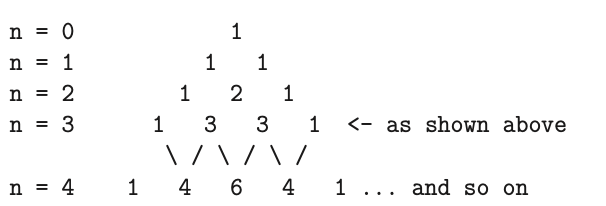
\includegraphics[scale=0.5]{imgs/pascal_triangle.png}
\end{figure}

\end{frame}


%------------------------------------------------------
\subsection{5.4.3 Catalan Numbers}

\begin{frame}[fragile]
\frametitle{Catalan Numbers}

The $n$-th Catalan number is defined as:

\begin{equation*}
    \text{Cat}(n) = \frac{C\binom{2n}{n}}{n+1}
\end{equation*}

$\text{Cat}(0) = 1$

\end{frame}

\begin{frame}[fragile]
\frametitle{Catalan Numbers}

For example, 

\begin{equation*}
    \text{Cat}(3) = \frac{C\binom{2\cdot3}{3}}{3+1} = \frac{20}{4} = 5
\end{equation*}

\end{frame}

\begin{frame}[fragile]
\frametitle{Catalan Numbers}

If we were asked to compute $n$ values of Catalan numbers we could use a bottom-up Dynamic Programming approach: if we know $\text{Cat}(n)$ we could compute $\text{Cat}(n+1)$ as follows:

\begin{equation*}
    \text{Cat}(n+1) = \frac{(2n+2)\cdot(2n+1)}{(n+2)\cdot(n+1)}\cdot \text{Cat}(n)
\end{equation*}

\end{frame}

\begin{frame}[fragile]
\frametitle{Catalan Numbers}

Catalan numbers are found in various combinatorial problems:

\begin{enumerate}
    \item $\text{Cat}(n)$ counts the number of distinct binary trees with $n$ vertices. For example, $n=3$
    	\vspace{0.15cm}
    	\begin{figure}
		    \centering
		    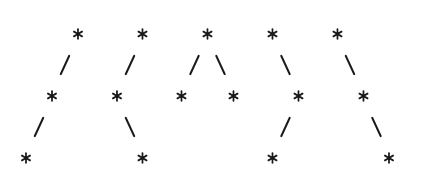
\includegraphics[scale=0.7]{imgs/catalan_binary_trees.png}
		\end{figure}
    \item $\text{Cat}(n)$ counts the number of expressions containing $n$ pairs of parentheses which are correctly matched. For example, $n=3$: \color{red} ()()(), ()(()), (())(), ((())), (()())\color{black}
\end{enumerate}

\end{frame}

\begin{frame}[fragile]
\frametitle{Catalan Numbers}

\begin{enumerate}
	\setcounter{enumi}{2}
    \item $\text{Cat}(n)$ counts the number of ways a convex polygon of $n + 2$ sides can be triangulated. A convex polygon is one in which all of its internal angles are equal or less than $180^\circ$ \color{blue}(left image)\color{black}
    \item $\text{Cat}(n)$ counts the number of monotonic paths along the edges of an n$ \times n$ grid, which do not pass above the diagonal. A monotonic path is one which starts in the lower left corner, finishes in the upper right corner, and consists entirely of edges pointing rightwards or upwards \color{blue}(right image)\color{black}
\end{enumerate}

\begin{figure}
    \centering
    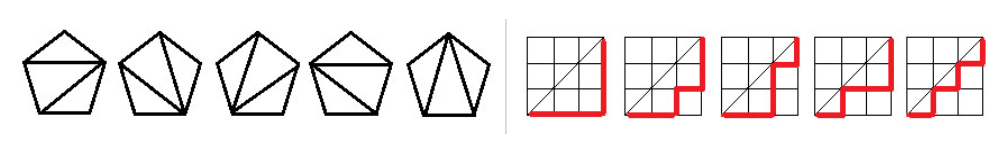
\includegraphics[scale=0.5]{imgs/catalan_2.png}
\end{figure}

\end{frame}

\begin{frame}[fragile]
\frametitle{Combinatronics in Programming Contests}

\begin{itemize}
    \item In online programming contests, if Internet access is allowed, one can generate small instances of a sequence and then search that sequence in the Online Encyclopedia of Integer Sequences (OEIS): \url{http://oeis.org/}
\end{itemize}

\end{frame}


\begin{frame}[fragile]
\frametitle{Combinatronics Problems}

\begin{itemize}
    \item \href{https://onlinejudge.org/index.php?option=com_onlinejudge&Itemid=8&category=713}{UVa - Combinatronics Problems}
    \item If site is down, please check \cite{Halim}: page 207-209 and browse for each problem at \href{https://cpbook.net/methodstosolve}{CP Book's Method to Solve}
\end{itemize}

\end{frame}



%------------------------------------------------------
%------------------------------------------------------
%------------------------------------------------------
\section{5.6 Probability Theory}

\begin{frame}[fragile]
\frametitle{Probability Theory}

\begin{quote}
    Branch of mathematics dealing with the analysis of random phenomena
\end{quote}

\vspace{0.3cm}

For certain random phenomena (such as toin cossing), the sequence of random events will exhibit -in the long term- a certain statistical pattern. For example, the probability of a head in a toss coin -in the long term- will be $1/2$

\end{frame}

\begin{frame}[fragile]
\frametitle{Probability Theory}

In programming contests, problems involving probability will be solvable with:

\begin{itemize}
    \item \textbf{Closed-form formula}: for these type of problems, we need to derive a formula (usually $O(1)$)
    \item \textbf{Exploration of the search space to count the number of events over the countable sample space}: these type of problems may involve some sort of Combinatronics, Complete Search of Dynamic Programming
\end{itemize}

\end{frame}

\begin{frame}[fragile]
\frametitle{Probability Theory Problems}

\begin{itemize}
    \item \href{https://onlinejudge.org/index.php?option=com_onlinejudge&Itemid=8&category=730}{UVa - Probability Theory}
    \item If site is down, please check \cite{Halim}: page 222 and then browse for the problem's PDF \href{https://cpbook.net/methodstosolve}{here}
\end{itemize}

\end{frame}


%------------------------------------------------------
%------------------------------------------------------
%------------------------------------------------------
\section{6.5 String Processing with Dynamic Programming}

\begin{frame}[fragile]
\frametitle{String Processing with Dynamic Programming}

Now, we'll study some string processing problems which solution can be found using Dynamic Programming techniques previously seen. 

\vspace{0.3cm}

Classical string processing problems every competitive programmer must know:
\begin{enumerate}
    \item String Alignment
    \item Longest Common Subsequence
\end{enumerate}

\vspace{0.3cm}

After studying these two problems, we'll study more problems that contain slight modifications of these two. 

\end{frame}

\begin{frame}
\frametitle{String Processing with Dynamic Programming}

\color{blue}\textbf{Note:} for various DP problems on string, we usually manipulate the integer indices of the strings and not the actual strings (or substrings) themselves. Passing substrings as parameters is very slow and hard to memoize \color{black}

\end{frame}


%------------------------------------------------------
\begin{frame}[fragile]
\frametitle{String Alignment (Edit Distance)}

\color{red}\textbf{Problem description}\color{black}

Align two strings $A$ with $B$ with the maximum alignment score (or minimum number of edit operations):

\begin{enumerate}
    \item Character $A[i]$ and $B[i]$ match: \textbf{+2 points}
    \item Character$ A[i$] and $B[i]$ mismatch and we replace $A[i]$ with $B[i]$: \textbf{-1 point}
    \item We insert a space in $A[i]$: \textbf{-1 point}
    \item We delete a letter from $A[i]$: \textbf{-1 point}
\end{enumerate}

\end{frame}

\vspace{0.3cm}

\begin{itemize}
    \item \color{red}\verb|C++ code: ch6_03_str_align.cpp|\color{black}
\end{itemize}

\begin{frame}[fragile]
\frametitle{String Alignment (Edit Distance)}

For example (non optimal alignment score),

\vspace{0.3cm}

\verb|A = 'ACAATCC'| $\rightarrow$ \verb|A_CAATCC| 

\verb|B = 'AGCATGC'| $\rightarrow$ \verb|AGCATGC_|

\color{blue}Alignment score = $4*2 + 4*(-1) = 4$\color{black}

\end{frame}

\begin{frame}[fragile]
\frametitle{String Alignment (Edit Distance)}

The solution for this problem is the Needleman-Wunsch's Bottom Up DP algorithm $O(nm)$: 

\begin{itemize}
    \item Consider two strings \verb|A[1..n]| and \verb|B[1..i]|
    \item $V(i,j)$: score of the optimal alignment between prefix \verb|A[1..i]| and \verb|B[1..j]|
    \item \textit{score}$(C1,C2)$: function that returns the score if the character $C1$ is aligned with character $C2$
\end{itemize}

\end{frame}

\begin{frame}[fragile]
\frametitle{String Alignment (Edit Distance)}

We define the following recurrences:

\vspace{0.3cm}
\textbf{Bases cases}:
\begin{itemize}
    \item $V(0,0) = 0$: no score for matching two empty strings
    \pause
    \item $V (i, 0) = i \times \text{score}(A[i], \_)$: '\_' represents an empty space, delete substring \verb|A[1..i]| to make the alignment $i>0$
    \pause    
    \item $V (0,j) = j \times \text{score}(\_, B[j])$: insert spaces \verb|B[1..j]| to make the alignment $i>0$
\end{itemize}

\pause
\vspace{0.3cm}
\textbf{Recurrences} for $i>0$ and $j>0$: 
\pause
\begin{itemize}
    \item $V (i, j) = \text{max}(\text{option1}, \text{option2}, \text{option3})$ where
    \pause
    \item option$1 = V(i-1, j-1) + \text{score}(A[i], B[j])$: score of match or mismatch
    \item option$2= V(i-1,j) + \text{score}(A[i], \_)$: delete $A_i$
    \item option$3= V(i,j-1) + \text{score}(\_, B[j])$: insert $B_j$
\end{itemize}

\end{frame}

\begin{frame}[fragile]
\frametitle{String Alignment (Edit Distance)}

\begin{figure}
    \centering
    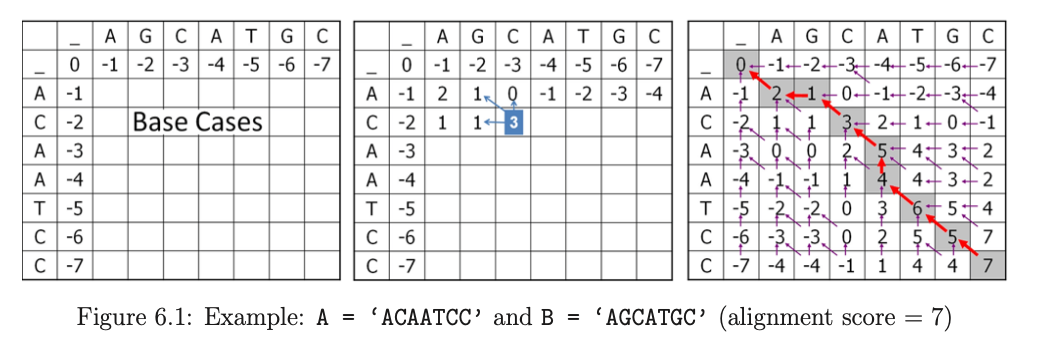
\includegraphics[scale=0.4]{imgs/string_alignment.png}
\end{figure}

\begin{itemize}
    \item Initially, only the base cases are known
    \item Then, we can fill the values row by row, left to right. To fill in $V(i,j) $for$ i,j > 0$, we just need three other values: $V(i-1,j-1)$, $V(i-1,j)$, and $V(i,j-1)$
   
\end{itemize}

\pause 

\vspace{0.3cm}
Optimal alignment:

\verb|A = 'A\_CAAT[C]C'|

\verb|B = 'AGC\_AT[G]C'|

\color{blue}Alignment score = $5*2 + 3*(-1) = 7$\color{black}

\end{frame}

%------------------------------------------------------
\begin{frame}[fragile]
\frametitle{Longest Common Subsequence}

\color{red}\textbf{Problem description}\color{black} 

Given two strings A and B, determine the longest common subsequence between them

\pause

\vspace{0.3cm}
For example, \verb|A = ‘ACAATCC’| and \verb|B = ‘AGCATGC’| have LCS of length $5$, i.e. \verb|‘ACATC’|


\end{frame}

\begin{frame}[fragile]
\frametitle{Longest Common Subsequence}

This LCS problem can be reduced to the String Alignment problem by setting the cost for mismatch as negative infinity, cost for insertion and deletion as 0, and the cost for match as 1. This makes the Needleman-Wunsch’s algorithm for String Alignment to never consider mismatches.

\end{frame}


%------------------------------------------------------
\begin{frame}[fragile]
\frametitle{Non Classical String Processing with DP}

\begin{itemize}
    \item \color{blue}UVa 11151 - Longest Palindrome\color{black}
\end{itemize}

\vspace{0.3cm}

\color{red}\textbf{Problem description}\color{black}

Given a string of up to $n = 1000$ characters, determine the length of the longest palindrome that you can make from it by deleting zero or more characters

\pause 
\vspace{0.3cm}

For example:

\begin{itemize}
    \item \verb|ADAM| $\rightarrow$ \verb|ADA|: length 3, delete \verb|M|
    \item \verb|MADAM| $\rightarrow$ \verb|MADAM|: length 5, delete nothing
\end{itemize}

\end{frame}

\begin{frame}[fragile]
\frametitle{UVa 11151}

DP solution $O(n^2)$: let \textit{len}$(l,r)$ be the length of the longest palindrome from string \verb|A[l..r]|

\vspace{0.3cm}

\pause
\textbf{Base cases}:

\begin{itemize}
    \item If \verb|l == r|, then \verb|len(l,r) = 1|, odd-length palindrome
    \item If \verb|l + 1 == r|:
    	\begin{itemize}
		    \item If \verb|A[l] == A[r]|, then \verb|len(l,r) = 2|
		    \item Otherwise, \verb|1|, even-length palindrome
		\end{itemize}
\end{itemize}

\pause 

\textbf{Recurrences}:
\begin{itemize}
    \item If \verb|A[l] == A[r]|, then \verb|len(l,r) = 2 + len(l+1, r-1)|, both corner characters are the same
    \item Otherwise, \verb|len(l,r) = max(len(l,r-1), len(l+1,r))|, increase left side or decrease right side
\end{itemize}

\end{frame}

\begin{frame}[fragile]
\frametitle{Problems}

\begin{itemize}
    \item \href{https://onlinejudge.org/index.php?option=com_onlinejudge&Itemid=8&category=751}{UVa - String Processing with DP: Classic}
        \item \href{https://onlinejudge.org/index.php?option=com_onlinejudge&Itemid=8&category=752}{UVa - String Processing with DP: Non Classic}
    \item If site is down, please check \cite{Halim}: page 248
\end{itemize}

\end{frame}


%------------------------------------------------------
%------------------------------------------------------
%------------------------------------------------------
\section{8.3 More Advanced DP Techniques}
\begin{frame}[fragile]
\frametitle{More Advanced DP Techniques}

Now, we'll look into more advanced DP techniques:

\begin{itemize}
    \item DP with Bitmask
    \item Compilation of common DP parameters
    \item Offset Technique
    \item Balanced BST as Memo Table
\end{itemize}

\end{frame}

%------------------------------------------------------
\subsection{8.3.1 DP with Bitmask}
\begin{frame}
\frametitle{}
\color{blue}
\centerline{\Large{8.3.1}}

\vspace{0.3cm} 

\centerline{\Large{DP with Bitmask}}
\color{black}
\end{frame}

\begin{frame}[fragile]
\frametitle{DP with Bitmask}

\begin{itemize}
    \item Some of the modern DP problems require a (small) set of Boolean as one of the parameters of the DP state
    \item Bitmask technique can be useful as one of the parameters in the DP table
\end{itemize}

\end{frame}


\begin{frame}[fragile]
\frametitle{UVa 10911 - Forming Quiz Teams}

\begin{itemize}
    \item \color{blue}\verb|C++ code: ch8_02_10911.cpp|\color{black}
\end{itemize}

\color{red}\textbf{Problem description}\color{black}

Let $(x, y)$ be the coordinates of a student’s house on a 2D plane. There are $2N$ students and we want to pair them into $N$ groups. Let $d_i$ be the distance between the houses of $2$ students in group $i$. Form $N$ groups such that \textit{cost} $ = \sum_{i=1}^{N}d_i$ is minimized. Output the minimum cost. Constraints: $1 \leq N \leq 8$ and $0 \leq x, y \leq 1000$

\begin{figure}
    \centering
    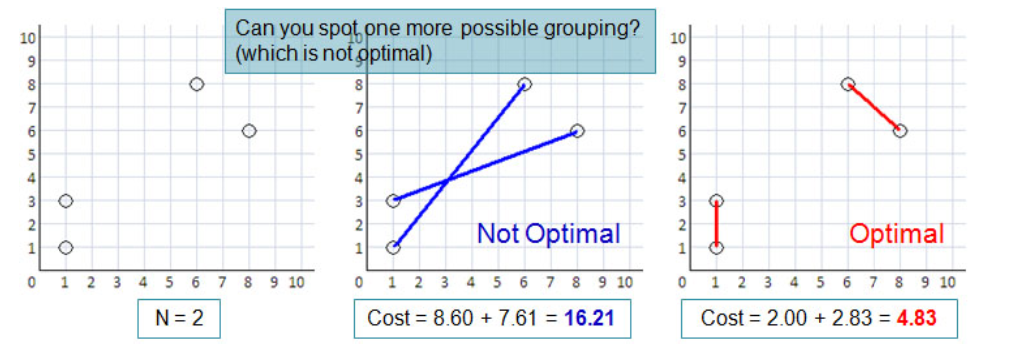
\includegraphics[scale=0.4]{imgs/uva_10911.png}
\end{figure}

\end{frame}

\begin{frame}[fragile]
\frametitle{UVa 10911 - Forming Quiz Teams}
\color{blue}*This problem is formally called: "minimum weight perfect matching on a small generated weighted graph". This is a \textbf{hard} problem but if $M \leq 20$ then DP bitmask solution can be used\color{black}
\end{frame}


\begin{frame}[fragile]
\frametitle{UVa 10911 - Forming Quiz Teams}

\textbf{For example}, when $M=6$, ($M=2N)$:

\begin{itemize}
    \item We start with a state where nothing is matched (\verb|bitmask = 000000|)
    
    \pause 
    \item If item $0$ and item $2$ are matched, we can turn on two bits (bit 0 and bit 2), thus the state becomes \verb|bitmask = 000101|
    
    \pause 
   	\item If from this state, item $1$ and item $5$ are matched next, the state will become \verb|bitmask = 100111|
	
	\pause 
	\item The perfect matching is obtained when the state is all ‘1’s, in this case: \verb|bitmask=111111|
\end{itemize}

\end{frame}

\begin{frame}[fragile]
\frametitle{UVa 10911 - Forming Quiz Teams}

\textbf{Solution}

\begin{itemize}
    \item There are only $O(2^M)$ distinct states. (Each number in the bitmask is a different state)
    \pause 
    \item For each state, we store the minimum weight of previous matchings that must be done in order to reach this state
    \pause 
    \item First, we find one ‘off’ bit $i$ using one $O(M)$ loop. Then, we find the best other ‘off’ bit $j$ from \verb|[i+1..M-1]| using another $O(M)$ loop and recursively match $i$ and $j$
    \pause
    \item This algorithm runs in $O(M\times 2^M)$
\end{itemize}

\end{frame}

%------------------------------------------------------
\subsection{8.3.2 Compilation of Common DP Parameters}
\begin{frame}
\frametitle{}
\color{blue}
\centerline{\Large{8.3.2}}
\vspace{0.3cm} 
\centerline{\Large{Compilation of Common DP Parameters}}
\color{black}
\end{frame}

\begin{frame}[fragile]
\frametitle{Compilation of Common DP Parameters}

\begin{enumerate}
    \item \textbf{Parameter:} Index $i$ in array $[x_0, x_1, \ldots, x_i, \ldots]$
\end{enumerate}

\end{frame}



%------------------------------------------------------
\subsection{8.3.3 Handling Negative Parameter Values with Offset Technique}

\begin{frame}
\frametitle{}
\color{blue}
\centerline{\Large{8.3.3}}
\vspace{0.3cm} 
\centerline{\Large{Handling Negative Parameter Values with Offset Technique}}
\color{black}
\end{frame}

\begin{frame}[fragile]
\frametitle{Handling Negative Parameter Values with Offset Technique}

\begin{itemize}
	\item In some cases, the DP parameter can go negative which causes an issue since most of the times we use this parameter as index in a DP table
    \item This can be solved using the \textbf{offset} technique
\end{itemize}

\end{frame}

\begin{frame}[fragile]
\frametitle{Handling Negative Parameter Values with Offset Technique}

\begin{itemize}
    \item \color{blue}UVa 1238 - Free Parentheses\color{black}
\end{itemize}

\vspace{0.3cm}

\color{red}\textbf{Problem description}\color{black} \\

Given an arithmetic expression which consists of only addition and subtraction operators, put any parentheses to the expression (as long as it's still valid), \textbf{how many different numbers can you make?}

\vspace{0.3cm}

\end{frame}

\begin{frame}[fragile]
\frametitle{UVa 1238 - Free Parentheses}

For example, $1 - 2 + 3 - 4 - 5$: 
\begin{columns}
\column{0.5\textwidth}

\begin{itemize}
    \item $1 - 2 + 3 - 4 - 5 = -7$
    \item $1 - (2 + 3) - 4 - 5 = -13$
    \item $1-(2+3-4)-5 = -5$
\end{itemize}

\column{0.5\textwidth}

\begin{itemize}
    \item $1 - (2 + 3 - 4 - 5) = 5$
    \item $1 - 2 + 3 - (4 - 5) = 3$
    \item $1-(2+3)-(4-5)= -3$
\end{itemize}

\end{columns}

\end{frame}

\begin{frame}[fragile]
\frametitle{UVa 1238 - Free Parentheses}

The expression consists of only $2 \leq N \leq 30$ non-negative numbers less than $100$ separated by addition or subtraction operators and there is no operator before the first and after the last number.

\vspace{0.3cm}

Let's look at the following remarks:

\begin{itemize}
    \item We only need to put a parentheses after a subtraction operator '-'
    \item We can only put $X$ closing parentheses if we have used $X$ open parentheses
    \item Maximum value: $100 + 100 + \ldots + 100 = 3000$
    \item Minimum value: $0 - 100 - \ldots - 100 = -2900$
\end{itemize}

\end{frame}

\begin{frame}[fragile]
\frametitle{UVa 1238 - Free Parentheses}

\textbf{Solution}

\vspace{0.3cm}

DP parameters:

\begin{enumerate}
    \item \verb|idx|:  current position in the expression being processed
    \item \verb|open|: number of open parentheses (we need this parameter to build a valid expression)
    \item \verb|val|: total value of the current expression
\end{enumerate}

\vspace{0.3cm}
\pause

\color{blue}*The memo table will consist of a 3D array \verb|visited[idx][open][idx+3000]| where the offset technique is represented by adding the maximum value to the current index \verb|idx|\color{black}

\end{frame}


%------------------------------------------------------
\subsection{8.3.4 MLE? Balanced BST as a Memo Table}
\begin{frame}
\frametitle{}
\color{blue}
\centerline{\Large{8.3.4}}
\vspace{0.3cm} 
\centerline{\Large{MLE? Balanced BST as a Memo Table}}
\color{black}
\end{frame}

\begin{frame}[fragile]
\frametitle{MLE? Balanced BST as a Memo Table}

Let's revisit the differences between Top-Down DP approach and Bottom-Up DP:

\begin{figure}
    \centering
    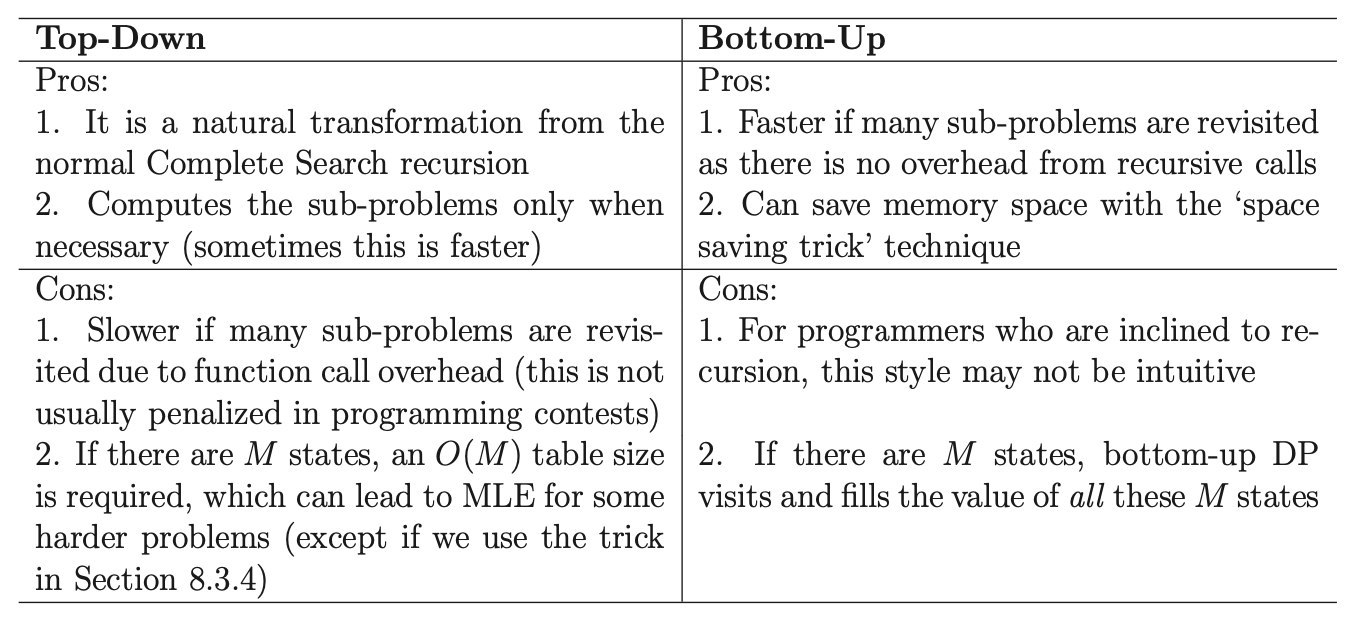
\includegraphics[scale=0.4]{imgs/td_vs_bu.png}
\end{figure}

\end{frame}

\begin{frame}[fragile]
\frametitle{MLE? Balanced BST as a Memo Table}

\begin{itemize}
    \item In previous slides, we've seen the Knapsack 0-1 problem where the state is \verb|(id, remW)|
    \item Parameter \verb|id| has a range of \verb|[0..n-1]| and parameter \verb|remW| a range of \verb|[0..S]|
    \item If the problem states that $n \times S$ is too large, the DP table of size $n\times S$ might result in a MLE (Memory Limit Exceeded) verdict
    
\end{itemize}

\end{frame}

\begin{frame}[fragile]
\frametitle{MLE? Balanced BST as a Memo Table}

\begin{itemize}
    \item If we run a Top-Down DP on this problem, not all of the states will be visited (in comparison to a Bottom-Up approach)
    \item We can trade runtime for smaller space by using a balanced BST (\verb|C++ STL map|) as the memo table
    \item This balanced BST will only store the states visited by the Top-Down DP
\end{itemize}

\vspace{0.3cm}

\color{blue}Thus, if there are only $k$ visited states, we'll only use $O(k)$ space instead of $O(n \times S)$\color{black}

\end{frame}

%------------------------------------------------------
\subsection{8.3.5 MLE/TLE? Use Better State Representation}

\begin{frame}
\frametitle{}
\color{blue}
\centerline{\Large{8.3.5}}
\vspace{0.3cm} 
\centerline{\Large{MLE/TLE? Use Better State Representation}}
\color{black}
\end{frame}

\begin{frame}[fragile]
\frametitle{MLE/TLE? Use Better State Representation}

If we coded a correct DP solution but the OJ still gives a MLE or TLE, we have no option but to use a better DP state representation in order to reduce the DP table size and speed the overall time complexity

\end{frame}

\begin{frame}[fragile]
\frametitle{MLE/TLE? Use Better State Representation}

\begin{itemize}
    \item \color{blue}UVa 1231 - ACORN\color{black}
    \item \color{red}\verb|C++ code: ch8_03_UVa1231.cpp|\color{black}
\end{itemize}

\vspace{0.3cm}

\color{red}\textbf{Problem description}\color{black} \\

Given $t$ oak trees, the height $h$ of \textbf{all} trees, the height $f$ that Jayjay the squirrel loses when it flies from one tree to another, $1 \leq t,h \leq 2000$, $1 \leq f \leq 500$, and the positions of acorns on each of the oak trees: \verb|acorn[tree][height]|, determine the max number of acorns that Jayjay can collect in one single descent. 

\end{frame}

\begin{frame}[fragile]
\frametitle{UVa 1231 - ACORN}

\textbf{For example}, $t=3$, $h=10$, $f=2$, the best descent has a total of $8$ acorns:

\begin{figure}
    \centering
    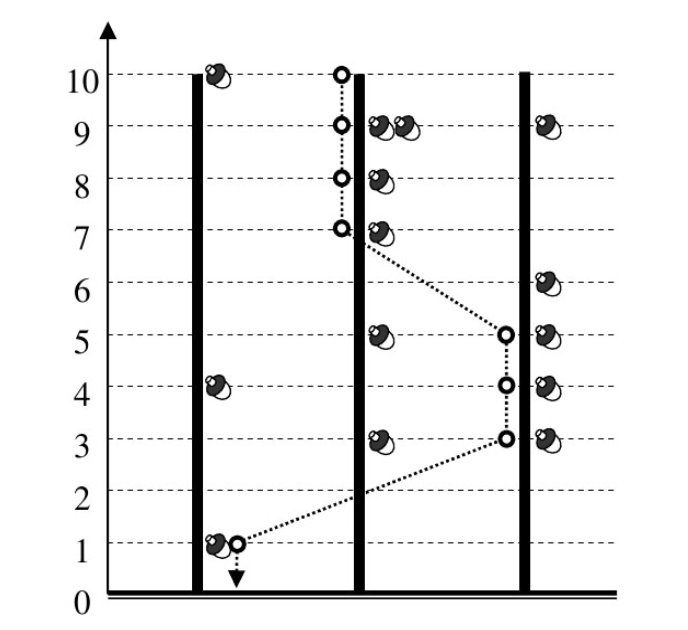
\includegraphics[scale=0.4]{imgs/uva_1231.png}
\end{figure}

\end{frame}

\begin{frame}[fragile]
\frametitle{UVa 1231 - ACORN}

\textbf{Naive DP Solution}:

\vspace{0.3cm}

\begin{itemize}
    \item Use a table \verb|total[tree][height]| that stores the best possible acorns collected when Jayjay is on a certain tree at certain height
    \item Jayjay recursively tries to either go down (-1) unit on the same oak tree or flies ($-f$) unit(s) to $t-1$ other oak trees from this position
    \item On the largest test case, this requires $2000 \times 2000 = 4M$ states and $4M \times 2000 = 8B$ operations
\end{itemize}

\vspace{0.3cm}

\color{blue}*This approach is clearly TLE\color{black}

\end{frame}

\begin{frame}[fragile]
\frametitle{UVa 1231 - ACORN}

\textbf{Best DP Solution}:

\vspace{0.3cm}

\begin{itemize}
    \item We can actually ignore the information: “On which tree Jayjay is currently at” as just memoizing the best among them is sufficient
    
    \pause
    \item This is because flying to any other $t-1$ other oak trees decreases Jayjay’s height in the same manner
    
    \pause
    \item \verb|dp[height]| will store the best possible acorns collected when Jayjay is at this height
    
    \item This Bottom-Up DP takes $2000 = 2K$ states and time complexity of $2000 \times 2000 = 4M$
\end{itemize}

\vspace{0.3cm}

\color{blue}*\verb|C++ code ch8_03_UVa1231.cpp|\color{black}

\end{frame}

\begin{frame}[fragile]
\frametitle{UVa 1231 - ACORN}

When the size of naive DP states are too large that causes the overall DP time complexity to be not doable, think of another more efficient (but usually not obvious) way to represent the possible states

\end{frame}


%------------------------------------------------------
\subsection{8.3.6 MLE/TLE? Drop One Parameter, Recover It From Others}

\begin{frame}
\frametitle{}
\color{blue}
\centerline{\Large{8.3.6}}
\vspace{0.3cm} 
\centerline{\Large{MLE/TLE? Drop One Parameter, Recover It From Others}}
\color{black}
\end{frame}

\begin{frame}[fragile]
\frametitle{MLE/TLE? Drop One Parameter, Recover It From Others}

Another trick to reduce the memory space and speed up the solution is to \color{blue}drop one important parameter \color{black} which can be recovered by using the other parameter(s)

\end{frame}


\begin{frame}[fragile]
\frametitle{MLE/TLE? Drop One Parameter, Recover It From Others}

\begin{itemize}
    \item \color{blue}UVa 1099 - Sharing Chocolate\color{black}
\end{itemize}

\vspace{0.3cm}

\color{red}\textbf{Problem Description}\color{black} \\ 

Given a big chocolate bar of size $1 \leq w, h \leq 100, 1 \leq n \leq 15$ friends, and the size request of each friend. Can we break the chocolate by using horizontal and vertical cuts so that each friend gets one piece of chocolate bar of his chosen size?

\end{frame}

\begin{frame}[fragile]
\frametitle{UVa 1099 - Sharing Chocolate}

\textbf{For example}, the size of the original chocolate bar is $w = 4$ and $h = 3$. If there are $n=4$ friends, each requesting a chocolate piece of size $\{6, 3, 2, 1\}$, respectively, then we can break the chocolate into $4$ parts using $3$ cuts:

\begin{figure}
    \centering
    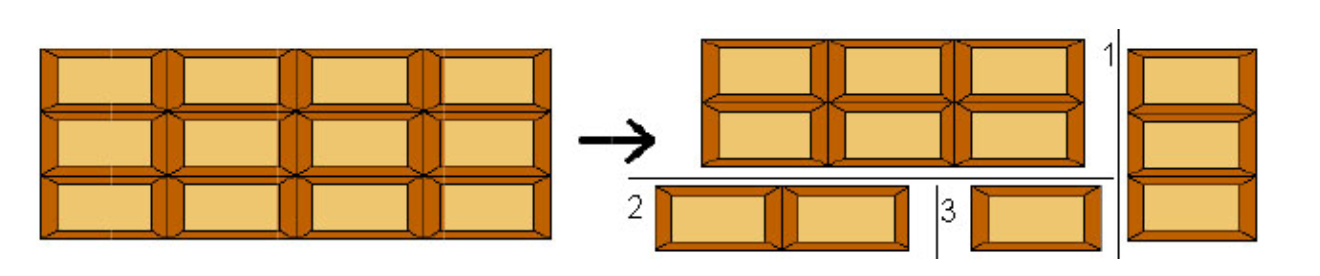
\includegraphics[scale=0.4]{imgs/uva_1099.png}
\end{figure}

\end{frame}

\begin{frame}[fragile]
\frametitle{UVa 1099 - Sharing Chocolate}

\textbf{One possible state representation}

\vspace{0.3cm}

\begin{itemize}
    \item State: \verb|(w, h, bitmask)|, where \verb|bitmask| is the subset of friends that already have a chocolate piece of their chosen size
	\item However, to implement this solution we'll need a DP table of size $100\times 2^15 = 327M$ which is \textbf{infeasible}
\end{itemize}

\end{frame}

\begin{frame}[fragile]
\frametitle{UVa 1099 - Sharing Chocolate}

\textbf{Better state representation}

\vspace{0.3cm}

\begin{itemize}
    \item Use only two parameters, either \verb|(w,bitmask)| or \verb|(h, bitmask)|
	\pause
	\item If we use \verb|(w,bitmask)|:
	\begin{itemize}
	    \item \verb|h = sum(bitmask) / w|
	\end{itemize}
	
	\pause
	\item DP table of size: $100\times 2^15 = 3M$ which is \textbf{reasonable}
\end{itemize}
\end{frame}

\begin{frame}[fragile]
\frametitle{UVa 1099 - Sharing Chocolate}

\textbf{Base cases}

\begin{itemize}
    \item If \verb|bitmask| only contains $1$ ‘on’ bit and the requested chocolate size of that person equals to $w \times h$, we have a solution
    \item Otherwise we do not have a solution.
\end{itemize}

\vspace{0.3cm}

\textbf{General case}

\begin{itemize}
    \item If we have a chocolate piece of size $w \times h$ and a current set of satisfied friends \verb|bitmask = bitmask1| U \verb|bitmask2|
    	\begin{itemize}
		    \item We can do either horizontal or vertical cut so that one piece is to serve friends in \verb|bitmask1| and the other is to serve friends in \verb|bitmask2|
		\end{itemize}
\end{itemize}

\end{frame}

%------------------------------------------------------
\begin{frame}[fragile]
\frametitle{UVa - Problems}

\begin{itemize}
    \item \href{https://onlinejudge.org/index.php?option=com_onlinejudge&Itemid=8&category=778}{UVa - More Advanced DP Techniques}
    \item If site is down, please refer to \cite{Halim}: page 318-319 and browse for the PDF's \href{https://cpbook.net/methodstosolve}{here}
\end{itemize}

\end{frame}


%------------------------------------------------------
%------------------------------------------------------
%------------------------------------------------------
\section*{References}
\begin{frame}{References}
    \begin{thebibliography}{}
        \bibitem[Halim]{Halim} Halim S., Halim F., \textit{Competitive Programming 3}, Handbook for ACM ICPC and IOI Contestants. 2013
        \bibitem[Skiean]{Skiena} Skiena S. \textit{The Algorithm Design Manual}. Springer. 2020
    \end{thebibliography}
\end{frame}

\end{document}
